% Created 2019-02-27 Wed 19:10
% Intended LaTeX compiler: pdflatex
\documentclass[11pt]{article}
\usepackage[utf8]{inputenc}
\usepackage[T1]{fontenc}
\usepackage{graphicx}
\usepackage{grffile}
\usepackage{longtable}
\usepackage{wrapfig}
\usepackage{rotating}
\usepackage[normalem]{ulem}
\usepackage{amsmath}
\usepackage{textcomp}
\usepackage{amssymb}
\usepackage{capt-of}
\usepackage{hyperref}
\author{Andrew Chen}
\date{\today}
\title{}
\hypersetup{
 pdfauthor={Andrew Chen},
 pdftitle={},
 pdfkeywords={},
 pdfsubject={},
 pdfcreator={Emacs 27.0.50 (Org mode 9.1.14)}, 
 pdflang={English}}
\begin{document}

\tableofcontents

\section{Things to Study For Quiz}
\label{sec:org9a4d9f8}

\subsection{Basic Vector and Matrix Operations}
\label{sec:orgf888579}

\subsubsection{Multiplication}
\label{sec:org50f55f8}

\begin{itemize}
\item Vector-Vector multiplication
\item Vector-Matrix multiplication
\item Matrix-Matrix multiplication
\item Matrix-Vector multiplication
\end{itemize}

\subsubsection{Finding Matrix Inverse}
\label{sec:org7fd45e4}

\begin{itemize}
\item For 2x2 Matrix:

If A =

\[\begin{bmatrix}
        a&b\\
        c&d\\
        \end{bmatrix}\]

A\(^{\text{-1}}\) =

1/det(A) *
\end{itemize}
\[\begin{bmatrix}
        d&-b\\
        -c&a\\
        \end{bmatrix}\]


\subsubsection{Determinant}
\label{sec:orgccc897d}

The factor by which a linear transformation changes the "area/volume" of a unit square/cube in a grid

If negative, then the unit square is "flipped" over its axis. (Like a square on paper after flipping the piece of paper)

\begin{itemize}
\item If A =

\[\begin{bmatrix}
     a&b\\
     c&d\\
     \end{bmatrix}\]
\end{itemize}


\textbf{\textbf{det(A) = ad - bc}}

\begin{itemize}
\item For calculating 3x3 matrices, go along the top row, and for a, b, c, cover the current row and column of a, b, c and multiply the a, b, c with the determinant of the uncovered numbers.
\begin{itemize}
\item For the "a" term, it's positive
\item For the "b" term, it's negative
\item For the "c" term, it's positive
\end{itemize}

\item If M =

\[\begin{bmatrix}
      a&b&c\\
      d&e&f\\
      g&h&i\\
      \end{bmatrix}\]

A = 
\[\begin{bmatrix}
      e&f\\
      h&i\\
      \end{bmatrix}\]

B = 
\[\begin{bmatrix}
      d&f\\
      g&i\\
      \end{bmatrix}\]

C = 
\[\begin{bmatrix}
      d&e\\
      g&h\\
      \end{bmatrix}\]

\textbf{\textbf{det(M) = a*det(A) - b*det(B) + c*det(C)}}
\end{itemize}

\subsubsection{Condition Number}
\label{sec:org3240eeb}

This is a measure of how much a small change in the transformation matrix or the output would affect the input vector

\begin{center}
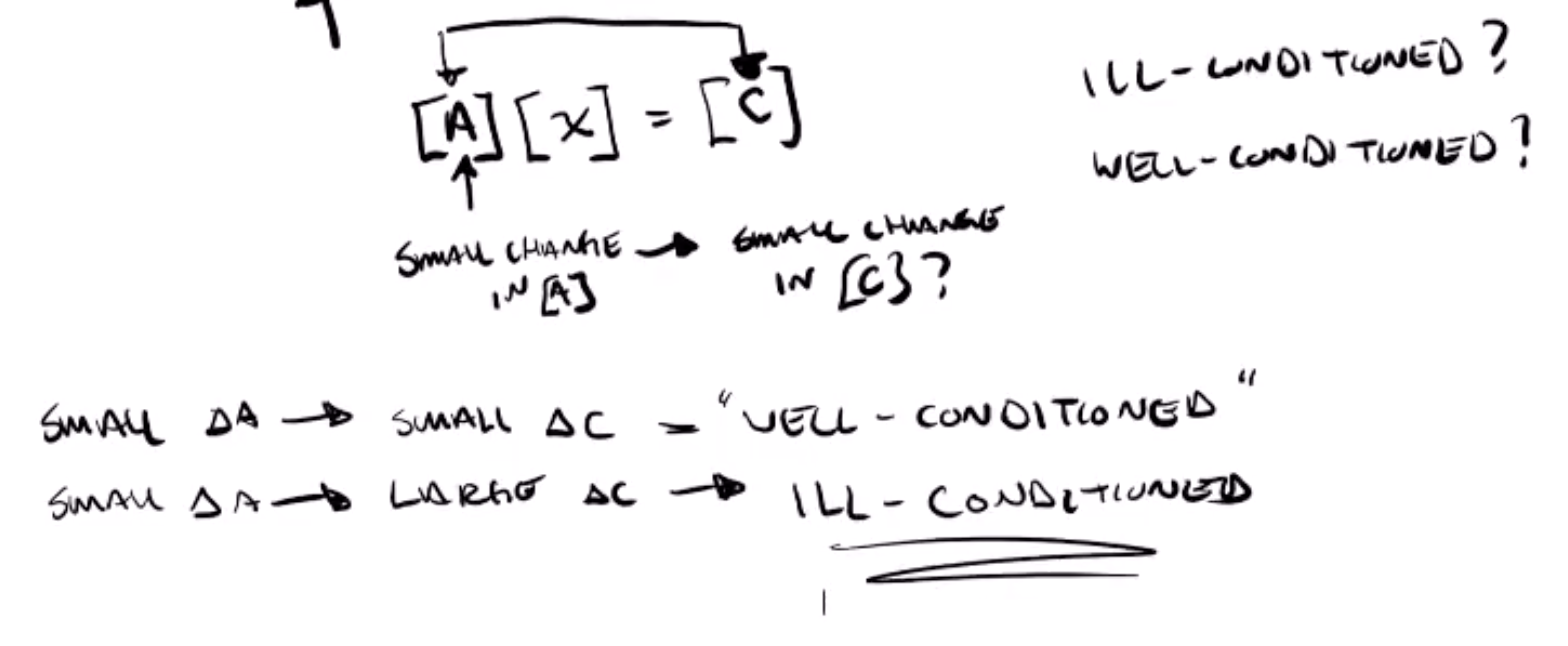
\includegraphics[width=.9\linewidth]{./images/condition1.png}
\end{center}
\begin{itemize}
\item If condition(A) \(\cong\) 1.0 \(\rightarrow\) "Well Conditioned"
\item If condition(A) > 1.0 \(\rightarrow\) "Ill Conditioned"
\item Condition(A): \(\kappa\)(A) = ||A|| * ||A\(^{\text{-1}}\)||
\end{itemize}

\subsection{Vector Norms}
\label{sec:orgda1f068}

\begin{itemize}
\item l\(_{\infty}\) Norm:

max\(_{\text{i}}\)|x\(_{\text{i}}\)|

\item l\(_{\text{p}}\) Norm:

\(\Sigma_{\text{i=1}}^{\text{n}}\) (|n|\(^{\text{p}}\))\(^{\text{1/p}}\)
\end{itemize}

\subsection{Vector Derivatives}
\label{sec:org2df3647}

\begin{itemize}
\item General Derivatives
\begin{center}
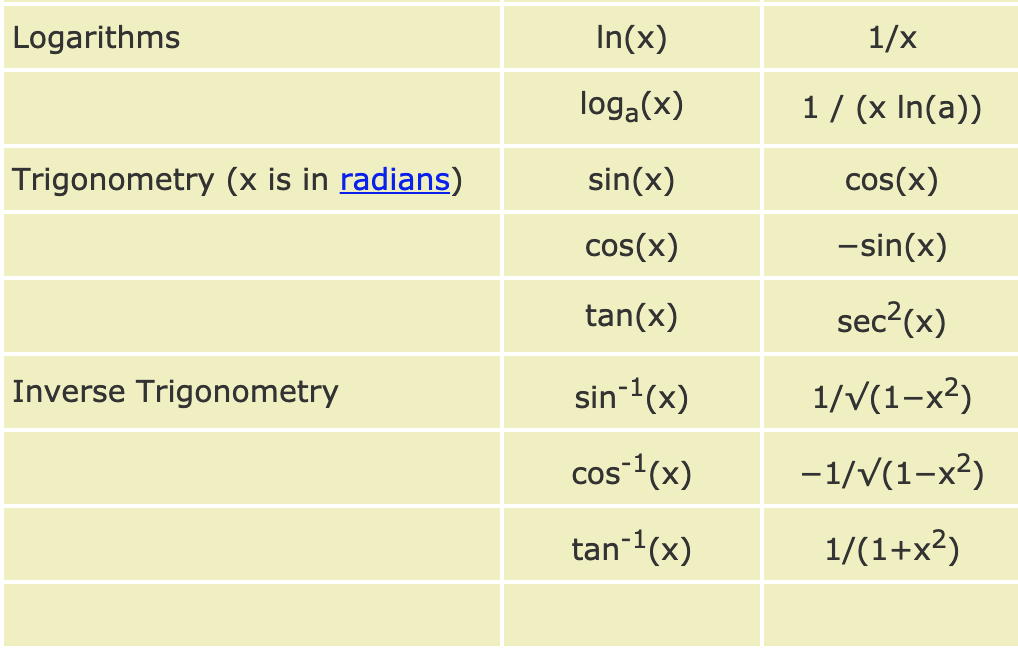
\includegraphics[width=.9\linewidth]{./images/derivatives.png}
\end{center}
\end{itemize}

\subsection{Machine Learning Basics}
\label{sec:orgee49312}

\begin{enumerate}
\item Regression
\item Classification
\item Clustering
\item Dimensionality Reduction
\item Activations functions (Logistic, ReLU, Leaky ReLU\ldots{})
\item Convex functions
\end{enumerate}

\subsection{Topics not on the Quiz}
\label{sec:org2064063}

\begin{itemize}
\item Neural Networks
\end{itemize}
\end{document}
